%%%%%%%%%%%%%%%
%
% $Autor: Wings $
% $Datum: 2020-01-29 07:55:27Z $
% $Pfad: General/SPI.tex
% $Version: 1785 $
%
%
%%%%%%%%%%%%%%%

	

\chapter{Schrittmotor}

In diesem Kapitel folgt eine grundsätzliche Beschreibung eines Schrittmotors. Darauf folgt die Erläuterungen zum Aufbau und Funktionsweise eines Schrittmotors sowie die Aufzählung verschiedener Grundbauarten. Nachfolgend werden Ursachen und Lösungen zum Verhindern von Schrittfehlern und der verwendete Schrittmotor genauer erläutert.

\section{Beschreibung eines Schrittmotors}

Ein Schrittmotor ist ein Elektromotor, der sich für präzise Positionierungsaufgaben eignet. Im Gegenteil zu anderen Elektromotoren wird bei einem Schrittmotor keine Positionsmessung oder Positionsregelung benötigt. Andere mechanische Antriebssysteme benötigen einen geschlossenen Regelkreis und mechanische Bremsen um Drehzahl und Position einzuhalten. Der Motor führt durch die Rotation des Rotors diskrete Schritte aus, wobei jeder Steuerimpuls eine Verschiebung um einen konstanten Winkel bewirkt. Mit diesem Motor ist eine erreichbare Positioniergenauigkeit von 0,1° möglich. Diese Art von Elektromotor wird beispielsweise in Druckern oder Scanner, aber auch im Kraftfahrzeugbereich verwendet. Im Kraftfahrzeugbereich werden die Schrittmotoren zur Spiegelverstellung sowie der Sitzverstellung verwendet. Das maximal erreichbare Drehmoment eines Schrittmotors liegt bei zwei Newtonmeter und die maximal erreichbare Drehzahl bei ca. 2000 Umdrehung pro Minute. Der Vorteil eines Schrittmotors ist die Wartungsfreiheit, da der Rotor keine Wicklungen hat. \cite{Babiel:2023,Hagl:2021,Bernstein:2018,Schroeder:2021}

\subsection{Aufbau und Funktionsweise eines Schrittmotors}

Der Schrittmotor besteht aus einem Stator, einem Rotor ohne Wicklungen und einer Steuerelektronik. Diese Steuerelektronik setzt sich zusammen aus einer Treiberstufe und der eigentlichen Steuerung. Bei dem Stator handelt es sich um den feststehenden äußeren Teil und bei dem Rotor um den beweglichen inneren Teil, wie in Abbildung \ref{HaPrSchritt} zu erkennen ist. Im Stator sind Spulen verbaut, die von einem Strom durchflossen werden. Hierdurch entsteht ein magnetisches Feld. Da der Rotor magnetisch ist, folgt er dem Magnetfeld des Stators. Soll eine Bewegung hervorgerufen werden, werden einzelne Wicklungsstränge ein- aus- oder umgeschaltet. Durch diesen Vorgang wird ein rotierendes Magnetfeld erzeugt. Das erzeugte Magnetfeld zieht den Rotor an. Der Rotor wird bei jedem Puls (Takt) um einen Winkelschritt weitergeschaltet. Die Anzahl der Polpaare im Stator geben die Anzahl der Schritte vor. Die Drehzahl und die Drehrichtung hängt von der Reihenfolge und der Häufigkeit der Stromimpulse ab. Es gibt drei verschiedene Betriebsarten, die abhängig von der Genauigkeit und der Drehzahl sind. Im Vollschrittbetrieb werden alle Polpaare bestromt. In dem Halbschrittbetrieb wird die Schrittzahl des Motors verdoppelt, wodurch sich die Positionsauflösung im Gegensatz zum Vollschrittbetrieb verdoppelt. Allerdings wird in diesem Betrieb das Drehmoment reduziert. In dem Mikroschrittbetrieb bewegt sich der Rotor in sehr kleinen Schritten. Hierdurch wird eine hohe Positioniergenauigkeit und ein ruhiger Lauf erreicht, da die Ströme und das Drehmoment in kleineren Schritten verändert werden. Bei einer zu hohen Schrittfrequenz kann ein Schrittverlust entstehen. Bei einem Schrittverlust überspringt der Motor einzelne Winkelschritte und landet in einer vorherigen oder nächsten Position gleicher Phase. Durch die offene Steuerkette werden die Verluste nicht erkannt.\cite{Hagl:2021,Bernstein:2018,Schroeder:2021}

\begin{figure}[H]
	\begin{center}
	%	\include{../../Images/Stepperdrive/StepperDriveTikz}
			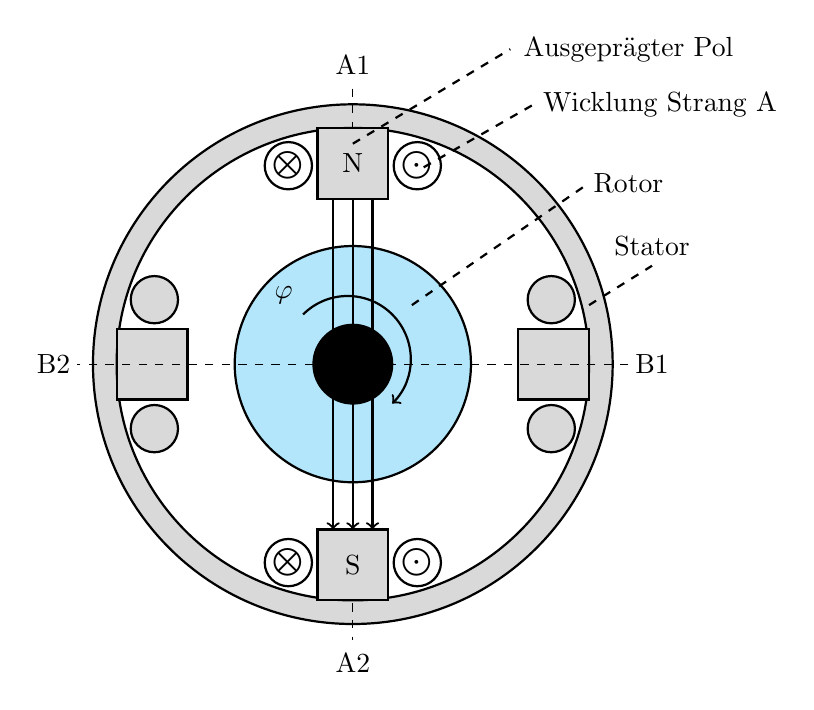
\begin{tikzpicture}
			% stator
			\draw[thick,fill=gray!30] (0,0) circle (3.3);
			\draw[thick, fill=white] (0,0) circle (3);
			
			% Achse
			\draw[dashed] (0,3.5) -- (0,-3.5);
			
			% Polung
			\draw[thick,fill=gray!30] (-0.45,3) rectangle (0.45,2.1) node[midway] {N};
			\draw[thick,fill=gray!30] (-0.45,-3) rectangle (0.45,-2.1) node[midway] {S};
			
			\draw[thick,fill=gray!30] (3,-0.45) rectangle (2.1,0.45) node[midway] {};
			\draw[thick,fill=gray!30] (-3,-0.45) rectangle (-2.1,0.45) node[midway] {};
			
			% rotor
			\filldraw[fill=cyan!30, thick] (0,0) circle (1.5);
			\filldraw[fill=black, thick] (0,0) circle (0.5);
			
			% Spulen
			\foreach \angle in {108, -108} {
				\draw[thick] (\angle:2.65) circle (0.3);
				\node at (\angle:2.65) {\small $\bigotimes$};
			}
			
			\foreach \angle in {72, -72} {
				\draw[thick] (\angle:2.65) circle (0.3);
				\node at (\angle:2.65) {\small $\bigodot$};
			}
			
			\foreach \angle in {18, -18, 162, -162} {
				\draw[thick, fill=gray!30] (\angle:2.65) circle (0.3);
				\node at (\angle:2.65) {};
			}
			
			% labels
			\node at (0,3.8) {A1};
			\node at (0,-3.8) {A2};
			\node at (3.8,0) {B1};
			\node at (-3.8,0) {B2};
			
			\node[align=center] at (3.5,4) {Ausgeprägter Pol};
			\draw[dashed,thick] (0,2.8) -- (2,4);
			
			\node[align=center] at (3.9,3.3) {Wicklung Strang A};
			\draw[dashed,thick] (0.9,2.5) -- (2.3,3.3);
			
			\node[align=center] at (3.5,2.3) {Rotor};
			\draw[dashed,thick] (0.75,0.75) -- (3,2.3);
			
			\node[align=center] at (3.8,1.5) {Stator};
			\draw[dashed,thick] (3,0.75) -- (3.8,1.25);
			
			% Magnetfeld
			\draw[->, thick] (0.25,2.1) -- (0.25,-2.1);
			\draw[->, thick] (0,2.1) -- (0,-2.1);
			\draw[->, thick] (-0.25,2.1) -- (-0.25,-2.1);
			
			% Achse
			\draw[dashed] (3.5,0) -- (-3.5,0);
			
			% phi
			\draw[<-, thick] (0.5,-0.5) arc[start angle=-45, end angle=135, radius=0.8] node[above left] {$\varphi$};
			
		\end{tikzpicture}
		
		\caption{Prinzipieller Aufbau Schrittmotor (2-phasig) \cite{Hagl:2021}} \label{HaPrSchritt}
	\end{center}
\end{figure}

\subsection{Schrittmotor Bauformen}

Wie bei anderen Elektromotoren gibt es auch bei dem Schrittmotor verschiedene Grundbauarten. 

\begin{itemize}
	\item {Permanentmagneterreger-Schrittmotor (PM-Schrittmotor)}
	\item {Reluktanzschrittmotor (VR-Schrittmotor)}
	\item {Hybridschrittmotor (Hybrid-Schrittmotor)}
\end{itemize}

Der \textbf{permanentmagnetische Schrittmotor} hat einen Permanentmagneten in dem Rotor verbaut. Hierbei stellt sich der permanentmagnetische Rotor immer so, dass der Nordpol des Rotors dem Nordpol des Statorfeldes gegenüber liegt und der Südpol des Rotors dem Südpol des Statorfeldes. In dieser Ausrichtung ziehen sich die Pole gegenseitig an. Die Drehrichtung des Rotors hängt von der Fließrichtung des Stromes ab. Der permanentmagnetische Schrittmotor entwickelt im ausgeschalteten Zustand ein Drehmoment zur Selbsthaltung. Dies ist aufgrund des permanentmagentischen Rotors möglich. Bei diesem Drehmoment handelt es sich um das höchste Drehmoment, das auf die Welle des Motors übertragen werden kann, ohne dass diese sich in eine rotierende Bewegung versetzt. Zu dieser Art von Schrittmotoren gehören beispielsweise der Klauenpol-Schrittmotor und der Scheibenmagnet-Schrittmotor. Bei der zweiten Bauart handelt es sich um den \textbf{Reluktanzschrittmotor}. Bei dieser Bauart besteht der Rotor aus einem weichmagentischen Material und besitzt eine gezahnte Form. So lange der Schrittmotor von keinem Strom durchflossen wird, entsteht kein Magnetfeld. Sobald der Motor in Betrieb genommen wird, entsteht ein magnetischer Fluss innerhalb des Rotors. Wird nun eine Wicklung erregt, wird der nächste Zahn des Rotors angezogen. Dadurch, dass die Rotorzähne ungleich der Polteilung sind, kann das System unendlich lange fortgesetzt werden. Die Anzahl der Schritte und die Genauigkeit des Reluktanzschrittmotors ist abhängig von der Anzahl der Zähne auf dem Rotor. Aus technischer Sicht sind mit dieser Bauart Schrittwinkel unter 1° möglich. Damit die Drehrichtung verändert werden kann, sind mindestens zwei Strangwicklungen nötig. Bei den \textbf{Hybridschrittmotoren}, auch bekannt als Hybridschrittmotoren handelt es sich um eine Kombination aus dem Reluktanzschrittmotor und dem Permanentmagneterreger-Schrittmotor. Durch diese Kombination aus den beiden Schrittmotoren werden die Vorteile aus der kleinen Schrittweite, dem hohen Drehmoment und dem Selbsthaltemoment genutzt. Bei dem Hybridschrittmotor besteht der Rotor aus zwei um eine halbe Zahnteilung versetzten weichmagnetischen Polrädern, die eine zahnförmige Form haben. Bei den beiden Polrädern bildet das eine Polrad den Nordpol und das zweite Polrad den Südpol. Zwischen den beiden Polrädern befindet sich ein Permanentmagnet. Anders als bei anderen Schrittmotoren wird der Rotor bei dieser Bauart axial magnetisiert. Damit ein kleiner Schrittwinkel möglich ist, haben die Statorpole ebenfalls eine zahnförmige Form. Die Ausrichtung des Rotors ist abhängig von der Stromrichtung und wird durch den minimalen Widerstand bestimmt, der sich aus dem Stromfluss durch die einzelnen Stränge ergibt. Wird ein besonders kleiner Schrittwinkel benötigt, kann dies durch Erhöhung der Zähnezahl erreicht werden. \cite{Schroeder:2021,Hagl:2021,Babiel:2023}

\subsection{Betriebsarten unipolar und bipolar}

Neben den oben bereits genannten Betriebsarten, kann außerdem zwischen dem Unipolarbetrieb und dem Bipolarbetrieb unterschieden werden. Der große Unterschied zwischen den beiden Betreibsarten besteht darin, dass in dem Unipolarbetrieb der Strom in eine Richtung fließt. Bei dem Bipolarbetrieb hingegen fließt der Strom in beide Richtungen. Dies ist möglich, da jeder Wicklungsstrang über eine Vollbrücke gespeist wird. Ein weiterer Unterschied besteht in der Schaltung der Zweige, durch die ein Gleichstrom fließt. In dem Unipolarbetrieb werden die beiden Zweige in Reihe geschaltet. Jeder Wicklungsstrang wird mit zwei Drähten parallel gewickelt. Sind die beiden Wicklungsstränge in dem Bipolarbetrieb parallel gewickelt, müssen die Zweige parallelgeschaltet werden. Im Bipolarbetrieb kann ein höherer Wirkungsgrad erzielt werden, wo hingegen der Unipolarbetrieb eine deutlich einfachere Schaltung aufweist. \cite{Schroeder:2021}

\subsection{Mikroschrittverfahren}

Mit dem Mikroschrittverfahren können Zwischenschritte und Mikroschritte erzeugt werden. Es bietet die Fähigkeit, Geräusche und Vibrationen zu minimieren sowie die Auflösung der Umdrehung zu erhöhen. Um Zwischenschritte zu erreichen, müssen beide Wicklungen eines Schrittmotors gleichzeitig mit Strom versorgt werden. 
Mit dem Sinus/Cosinus-Mikroschrittverfahren können die Mikroschrittverfahren realisiert werden, indem der Strom in jeder Phase des Motors sinusförmig variiert. Durch die Anwendung sinusförmiger Ströme auf die Motorwicklungen wird eine feinere und gleichmäßigere Bewegung erzielt, was zur einer präziseren Steuerung und reduzierten mechanischen Vibrationen führt.\cite{McComb:2024}

Ein Mikroschritt-Treiber unterteilt die Motorschrittwinkel in vier oder mehr Teil. Es handelt sich um einen Controller, der die Methode der Stromreglung verwendet, um die Mikroschritte zu erzeugen. Der Controller bietet außerdem den Vorteil einer erhöhten Flexibilität bei der Integration der Strombegrenzung und der Anpassung der Antriebscharakteristik als Reaktion auf Änderungen der Systemdynamik. Die Anzahl der Unterteilungen ist einstellbar, was eine präzise Steuerung und Anpassung an spezifische Anforderungen ermöglicht.\cite{Babiel:2023}

\section{Schrittverluste verhindern}
Um mögliche Schrittverlusten einzugrenzen und oder sie zu verhindern, wird in diesem Kapitel beschrieben, wie die Ursachen für Schrittverluste oder Stillstand methodisch zu ermitteln sind. \cite{Faulhaber:2020}

\subsection{Auswahl des Schrittmotors}
Zunächst muss ein passender Motor für die Anwendung gewählt werden. Dabei sollten folgende grundlegende Regeln erfüllt sein:
\begin{itemize}
	\item Motorauswahl durch Höchstwerte für Drehmoment und Drehzahl (Worst-Case-Szenario)
	\item Verwendung eines Sicherheitsaufschlag von 30 \% auf die Drehmoment-Drehzahl-Kennlinie(Kippmoment)
	\item Sicherstellen, dass externe Ereignisse die Anwendung nicht blockieren können
\end{itemize}

Sind die geforderten Drehmomente bei den jeweiligen Drehzahlen, den Motorspezifikation entsprechend, dann sind keine Probleme zu erwarten. Ist der Motor zu schwach gewählt und die Anwendung fordert mehr Leistung als der Motor abgeben kann, so bleibt der Motor stehen. Der nächste Schritt ist die Durchführung von Testdurchläufen. Es soll im Betrieb überprüft werden, ob Schrittverluste auftreten. Schrittmotoren verlieren konstruktionsbedingt nicht nur einen einzigen Schritt. Bei geringen Drehzahlen verliert der Motor ein Vielfaches von vier Schritten.\cite{Faulhaber:2020}


\subsection{Betriebsart}

In diesem Abschnitt werden je nach Betriebsart mögliche Ursachen erläutert, falls der Schrittmotor bei den Tests versagt.

\subsubsection{Start-Stopp-Betrieb}

Der Motor ist mit der Last fest verbunden und wird mit konstanter Drehzahl betrieben. Innerhalb des ersten Schrittes muss der Motor auf die vorgegebene Frequenz beschleunigen wie in Abbildung \ref{Start-Stopp Frequenz} zu sehen ist.\cite{Faulhaber:2020} 

\begin{figure}[!ht]
	\centering
	\resizebox{1\textwidth}{!}{%
		\begin{circuitikz}
			\tikzstyle{every node}=[font=\LARGE]
			\draw [line width=1pt, ->, >=Stealth] (11.25,8.25) -- (11.25,22);
			\draw [ color={rgb,255:red,0; green,199; blue,252}, line width=1pt, short] (36.25,12) -- (36.25,8.25);
			\node [font=\LARGE] at (38.75,7.5) {Zeit};
			\node [font=\huge] at (8.75,12.25) {f};
			\node [font=\LARGE] at (9.75,22) {Frequenz};
			\node [font=\normalsize] at (10,12) {Start/Stopp};
			\draw [ color={rgb,255:red,0; green,199; blue,252}, line width=1pt, short] (17.5,12) -- (17.5,8.25);
			\draw [line width=1pt, ->, >=Stealth] (11.25,8.25) -- (38.75,8.25);
			\draw [ color={rgb,255:red,0; green,199; blue,252}, line width=1pt, short] (17.5,12) -- (36.25,12);
			\draw [line width=1pt, dashed] (11.25,12) -- (17.5,12);
		\end{circuitikz}
	}%
	
	\caption{Start-Stopp Frequenz \cite{Faulhaber:2020}} \label{Start-Stopp Frequenz}
\end{figure}

{\textbf{Fehlerbild: Motor läuft nicht an (siehe Ursachen und Lösungen aus Tabelle \ref{MOTLNA})} 
	\begin{figure}
		\begin{center}
			\fontsize{8}{10}\selectfont
			\begin{tabularx}{\textwidth}{|X|X|X|X|X|X|}
				\hline 
				\textbf{Ursachen} & \textbf{Lösungen} \\ \hline
				Last zu Hoch & Falscher Motor, größeren Motor wählen \\ \hline
				Frequenz zu hoch & Frequenz reduzieren\\ \hline
				Pendelt der Motor von Links nach Rechts & Es könnte eine Phase unterbrochen oder nicht angeschlossen sein, dies muss repariert werden \\ \hline
				Phasenstrom passt nicht & Phasenstrom erhöhen\\ \hline
				
			\end{tabularx}
			\captionof{table}{Ursachen und Lösungen: Motor läuft nicht an \cite{Faulhaber:2020}} \label{MOTLNA} 
		\end{center}
	\end{figure}
	
	
	\subsubsection{Beschleunigung und Rampenprofil (Trapezförmig)}
	
	Der Motor kann mit einer im Controller vorgegebenen Beschleunigungsrate bis auf die Maximalfrequenz beschleunigen wie in Abbildung \ref{Trapezförmiges Geschwindigkeitsprofil} zu sehen ist.\cite{Faulhaber:2020} 
	
	\begin{figure}[!ht]
		\centering
		\resizebox{1\textwidth}{!}{%
			\begin{circuitikz}
				\tikzstyle{every node}=[font=\LARGE]
				\draw [line width=1pt, ->, >=Stealth] (11.25,8.25) -- (11.25,22);
				\draw [ color={rgb,255:red,0; green,199; blue,252}, line width=1pt, short] (17.5,12) -- (22.5,19.5);
				\draw [ color={rgb,255:red,0; green,199; blue,252}, line width=1pt, short] (22.5,19.5) -- (27.5,19.5);
				\draw [ color={rgb,255:red,0; green,199; blue,252}, line width=1pt, short] (27.5,19.5) -- (36.25,12);
				\draw [ color={rgb,255:red,0; green,199; blue,252}, line width=1pt, short] (36.25,12) -- (36.25,8.25);
				\draw [line width=1pt, dashed] (11.25,19.5) -- (22.5,19.5);
				\draw [line width=1pt, dashed] (27.5,19.5) -- (38.75,19.5);
				\draw [line width=1pt, dashed] (22.5,19.5) -- (22.5,8.25);
				\draw [line width=1pt, dashed] (27.5,19.5) -- (27.5,8.25);
				\draw [line width=1pt, dashed] (11.25,12) -- (38.75,12);
				\node [font=\LARGE] at (38.75,7.5) {Zeit};
				\node [font=\LARGE] at (19.25,7.75) {t};
				\node [font=\huge] at (32.5,7.75) {t};
				\node [font=\huge] at (8.75,12.25) {f};
				\node [font=\huge] at (9.75,19.75) {f};
				\node [font=\LARGE] at (9.75,22) {Frequenz};
				\node [font=\normalsize] at (19.75,7.5) {acc};
				\node [font=\normalsize] at (33,7.5) {dec};
				\node [font=\normalsize] at (10,12) {Start/Stopp};
				\node [font=\normalsize] at (10.25,19.5) {max};
				\draw [ color={rgb,255:red,0; green,199; blue,252}, line width=1pt, short] (17.5,12) -- (17.5,8.25);
				\draw [line width=1pt, ->, >=Stealth] (11.25,8.25) -- (38.75,8.25);
			\end{circuitikz}
		}%
		\caption{Trapezförmiges Geschwindigkeitsprofil \cite{Faulhaber:2020}} \label{Trapezförmiges Geschwindigkeitsprofil}
	\end{figure}
	
	
	{\textbf{Fehlerbild: Motor beendet die Beschleunigungsrampe nicht (siehe Ursachen und Lösungen aus Tabelle \ref{Beschleunigungsrampe})}
		\begin{center}
			\fontsize{8}{10}\selectfont
			\begin{tabularx}{\textwidth}{|X|X|X|X|X|X|}
				\hline 
				\textbf{Ursachen} & \textbf{Lösungen} \\ \hline
				
				Motor bleibt bei der Resonanzfrequenz hängen & 
				\begin{itemize} 
					\item {Beschleunigung erhöhen, um die Resonanzfrequenz schneller zu durchlaufen} 
					\item {Start-Stopp Frequenz über dem Resonanzpunkt wählen} 
					\item {Halbschritt- oder Mikroschrittbetrieb verwenden} 
					\item {Mechanische Dämpfung vorsehen} 
				\end{itemize}	 \\	\hline
				Falsche Einstellung von Versorgungsspannung oder Strom zu gering & 
				\begin{itemize}
					\item {Spannung oder Strom erhöhen} 
					\item {Motor mit geringerer Impedanz testen} 
					\item {Stromregelung verwenden}
				\end{itemize}\\	\hline
				Maximaldrehzahl zu hoch & 
				\begin{itemize}
					\item {Maximaldrehzahl reduzieren} 
					\item {Beschleunigungsrampe abflachen}
				\end{itemize}\\ \hline
				Schlechte Vorgabe der Beschleunigungsrampe durch Elektronik & 
				\begin{itemize}
					\item {Anderen Controller verwenden }
				\end{itemize}\\ \hline
			\end{tabularx}
			\captionof{table}{Ursachen und Lösungen: Motor beendet die Beschleunigungsrampe nicht \cite{Faulhaber:2020}}
			\label{Beschleunigungsrampe}	
		\end{center}
		
		{\textbf{Fehlerbild: Motor beschleunigt bis zur Enddrehzahl und bleibt stehen, sobald eine konstante Drehzahl erreicht ist (siehe Ursachen und Lösungen aus Tabelle \ref{stehenderMotor})}
			\begin{center}
				\fontsize{8}{10}\selectfont
				\begin{tabularx}{\textwidth}{|X|X|X|X|X|X|}
					\hline 
					\textbf{Ursachen} & \textbf{Lösungen} \\ \hline
					
					Motor wird an Leistungsgrenze betrieben und bleibt stehen aufgrund zu hoher Beschleunigung & 
					\begin{itemize} 
						\item {Ruckeln verringern durch geringere Beschleunigungsrate oder durch unterschiedliche Beschleunigungsrampen, erst steil dann flacher} 
						\item {Drehmoment erhöhen} 
						\item {Motor im Mikroschrittbetrieb betreiben} 
						\item {Mechanische Dämpfung vorsehen} 
					\end{itemize}	 \\	\hline
				\end{tabularx}
				\captionof{table}{Ursachen und Lösungen: Motor beschleunigt bis zur Enddrehzahl und bleibt stehen, sobald eine konstante Drehzahl erreicht ist. \cite{Faulhaber:2020}}
				\label{stehenderMotor}
			\end{center}
			
			
			
			\subsection{Externe Ereignisse}
			
			\subsubsection{Lastrückkopplung}
			
			\textit{\glqq Manchmal wird der vom Motor angetriebene Mechanismus/Last während der Bewegung \glqq aufgezogen \grqq und gibt diese Energie wieder an den Motor zurück, wenn die Ströme ausgeschaltet werden. Der Mechanismus könnte z.B. ein Untersetzungsgetriebe sein.\grqq}\cite{Faulhaber:2020} 
			Wird diese Energie an den Motor zurück geleitet, kann es passieren, dass der Motor sich um einen Winkel verdreht, der mehr als einem Schritt entspricht. Dabei kann es passieren, dass der Motor nicht ausreichend Drehmoment entwickelt und nicht oder erst nach 4 Vollschritten anläuft. \cite{Faulhaber:2020}
			
			\textbf{Lösungen:}
			\begin{itemize}
				\item Die Kommutierung so programmieren, dass Wert und Polarität vor dem Abschalten gespeichert und beim Wiedereinschalten verwenden werden kann. 
				\item Nicht vollständig den Strom abschalten, sondern bei Motorstillstand einen reduzierten \textit{Stand-By} Strom aufrechterhalten
			\end{itemize}
			
			\subsubsection{Erhöhung der Nutzlast mit der Zeit}
			\textit{\glqq Manchmal läuft der Motor für eine lange Zeit störungsfrei und viel später treten die ersten Schrittverluste auf. In diesem Fall ist es sehr wahrscheinlich, dass die Last, die der Motor „sieht“, sich geändert hat. Das kann auf Verschleiß der Motorlager oder ein externes Ereignis zurückzuführen sein.\grqq}\cite{Faulhaber:2020}
			
			\textbf{Lösungen:}
			\begin{itemize}
				\item Prüfen ob ein externes Ereignis durch Veränderung des Mechanismus vorliegt.
				\item Prüfen ob Lagerverschleiß vorhanden ist. Verwendung von Kugellager erhöhen die Lebensdauer des Motors.
				\item Verwendung von Schmiermittel um Reibung zu verhindern.
			\end{itemize}
			
			
			\section{Beschreibung des verwendeten Schrittmotors}
			
			Für das Automatisierungsprojekt wird ein Nema 17 Schrittmotor der Firma Creality3D verwendet. Dieser Schrittmotor wird im 3D-Druck sowie in CNC-Maschinen eingesetzt. Der Motor arbeitet im Bipolarbetrieb und es sind zwei Spulen verbaut. Er hat einen Schrittwinkel von 1,8 ° und benötigt 200 Schritte für eine volle Umdrehung. Die Wellenlänge beträgt 20 mm und der Wellendurchmesser 5 mm. Der ausgewählte Schrittmotor arbeitet mit einer Nennspannung von 12 Volt. Der Motor ist nicht für große Drehmomente ausgelegt, sondern für schnelle und präzise Bewegungen.  Dies wird qualitativ in der Abbildung \ref{DrehmomentDiagramm} für den Schrittmotor GM42BYG015 dargestellt. Hier ist zu erkennen, dass der Schrittmotor ein Drehmoment von ca. 0,8 kg$\cdot$cm erreicht. Auf der x-Achse wird die Geschwindigkeit in Pulses per Second (PPS) angegeben, d.h. die Anzahl der Steuerimpulse pro Sekunde. Der Schrittmotor erzielt aber eine gute Positioniergenauigkeit durch den kleinen Schrittwinkel und die Microstepp-Funktion. Des weiteren arbeitet der Motor mit 0,84 Amper pro Phase. Weitere Vorteile des Schrittmotors sind die kompakte Bauform mit den Abmessung $42\times 42\times 34$ mm sowie die geringe Masse mit 220 Gramm. Betrieben werden kann der Schrittmotor in einer Umgebungstemperatur von -10\ °C bis +50\ °C.\cite{Gems:2014,Gems:2022}
			
			\begin{figure}[H]
				\centering
	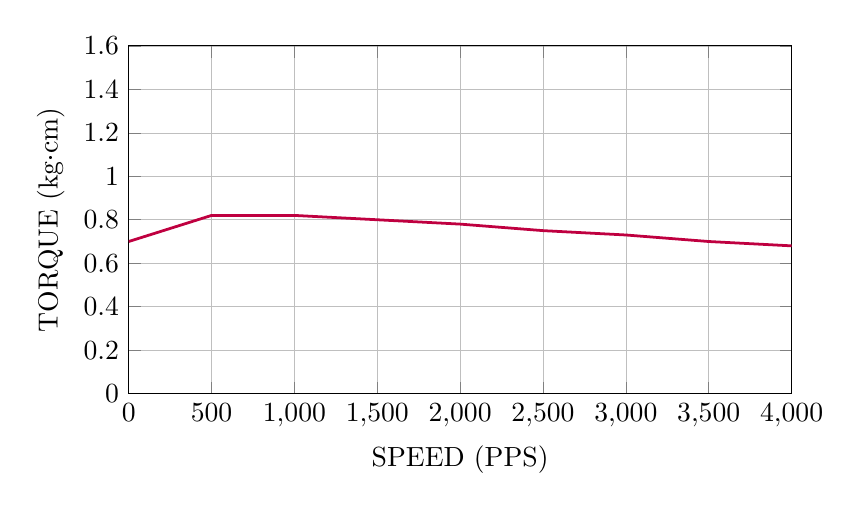
\begin{tikzpicture}
	\begin{axis}[
		width=10cm,
		height=6cm,
		xlabel={SPEED (PPS)},
		ylabel={TORQUE (kg·cm)},
		xmin=0, xmax=4000,
		ymin=0, ymax=1.6,
		xtick={0,500,1000,1500,2000,2500,3000,3500,4000},
		ytick={0,0.2,0.4,0.6,0.8,1,1.2,1.4,1.6},
		legend pos=north east,
		grid=both,
		major grid style={line width=.2pt,draw=gray!50},
		minor grid style={line width=.1pt,draw=gray!20},
		]
		\addplot[
		color=purple,
		line width=1pt
		]
		coordinates {
			(0,0.7)
			(500,0.82)
			(1000,0.82)
			(1500,0.8)
			(2000,0.78)
			(2500,0.75)
			(3000,0.73)
			(3500,0.7)
			(4000,0.68)
		};
	\end{axis}
\end{tikzpicture}
%				\input{tikz/MomentenverlaufSchrittmotor}
				\caption{Drehmoment-Diagramm für den Schrittmotor 42BYG015 \cite{Gems:2014}}
				\label{DrehmomentDiagramm}
			\end{figure}

			

\section{Beschreibung des Programms auf dem Arduino}

\subsection{Aufgabe des Programms}
Das Programm steuert einen Schrittmotor und zeigt Informationen auf einem OLED-Display an. Es nutzt einen Drehwinkel-Encoder, um verschiedene Betriebsstufen des Motors auszuwählen.

\begin{figure}[H]
	\begin{center}
\resizebox{\textwidth}{!}{%
	\begin{tikzpicture}[
		node distance=0.8cm and 1.5cm,
		startstop/.style={circle, draw, minimum size=1cm},
		process/.style={rectangle, draw, text width=2.7cm, align=center},
		decision/.style={diamond, draw, text width=2cm, align=center},
		arrow/.style={->, thick}
		]
		
		% Nodes
		\node (start) [startstop] {Start};
		\node (init) [process, below=of start] {Initialisierung};
		\node (display) [process, below=of init] {Display-Start};
		\node (status) [process, below=of display] {Status: Bereit};
		\node (wait) [process, below=of status] {Warten auf Eingabe};
		\node (enc_turned) [decision, below=of wait] {Encoder gedreht?};
		\node (button_pressed) [decision, right=of enc_turned, xshift=1.5cm] {Taster gedrückt?};
		\node (enc_left) [process, below left=of enc_turned, xshift=1cm] {Encoder links};
		\node (enc_right) [process, below right=of enc_turned, xshift=-1cm] {Encoder rechts};
		\node (stage_gt1) [decision, below=of enc_left] {Stufe > 1};
		\node (stage_lt10) [decision, below=of enc_right] {Stufe < 10};
		\node (stage_dec) [process, below=of stage_gt1] {Stufe -1};
		\node (stage_inc) [process, below=of stage_lt10] {Stufe +1};
		\node (update1) [process, below=of stage_dec] {Display aktualisiert};
		\node (update2) [process, below=of stage_inc] {Display aktualisiert};
		\node (ref_run) [process, below right=of button_pressed, xshift=-1cm] {Referenzfahrt};
		\node (end_pressed) [decision, below=of ref_run] {Endschalter?};
		\node (demo_run) [process, below=of end_pressed] {Demonstrations- fahrt};
		\node (display_run) [process, below=of demo_run] {Display: wird ausgeführt};
		\node (shuttle_move) [process, below=of display_run] {Schlitten pendelt};
		\node (display_ready) [process, below=of shuttle_move] {Display: Startbereit};
		
		% Arrows
		\draw [arrow] (start) -- (init);
		\draw [arrow] (init) -- (display);
		\draw [arrow] (display) -- (status);
		\draw [arrow] (status) -- (wait);
		\draw [arrow] (wait.south) -- ++(0,-0.5) -| (enc_turned.north);
		\draw [arrow] (wait.south) -- ++(0,-0.5) -| (button_pressed.north);
		\draw [arrow] (enc_turned) -- (enc_left);
		\draw [arrow] (enc_turned) -- (enc_right);
		\draw [arrow] (enc_left) -- (stage_gt1);
		\draw [arrow] (enc_right) -- (stage_lt10);
		\draw [arrow] (stage_gt1) -- (stage_dec);
		\draw [arrow] (stage_lt10) -- (stage_inc);
		\draw [arrow] (stage_dec) -- (update1);
		\draw [arrow] (stage_inc) -- (update2);
		\draw [arrow] (update1.south) -- ++(0,-0.5) -| ++(-5,0) |- (wait.west);
		\draw [arrow] (update2.south) -- ++(0,-0.5) -| ++(-8,0) |- (wait.west);
		\draw [arrow] (button_pressed) -- (ref_run);
		\draw [arrow] (ref_run) -- (end_pressed);
		\draw [arrow] (end_pressed) -- (demo_run);
		\draw [arrow] (demo_run) -- (display_run);
		\draw [arrow] (display_run) -- (shuttle_move);
		\draw [arrow] (shuttle_move) -- (display_ready);
		\draw [arrow] (display_ready.east) -- ++(1.5,0) |- (wait.east);
	\end{tikzpicture}
} % end resizebox
		\caption{Flussdiagramm des Programms}
		\label{fluss}
	\end{center}
\end{figure}

Beim Start des Programms werden alle Komponenten, einschließlich des Schrittmotors, des Displays, der LEDs und des Encoders, initialisiert. Nach einer kurzen Startanimation auf dem Display wechselt das System in den Bereitschaftsmodus. Der Benutzer kann den Drehwinkel-Encoder drehen, um eine der zehn verfügbaren Stufen auszuwählen. Jede Stufe hat spezifische Geschwindigkeitswerte für den Schrittmotor. Die aktuell ausgewählte Stufe wird auf dem OLED-Display angezeigt, sodass der Benutzer immer über die gewählte Einstellung informiert ist. Ein Taster ermöglicht es dem Benutzer, den Startprozess des Schrittmotors zu initiieren. Nach dem Drücken des Tasters führt der Schrittmotor Bewegungen aus, die der ausgewählten Stufe entsprechen. Diese Bewegungen beinhalten das Fahren zu einem festgelegten Punkt und das anschließende Zurückfahren zur Ausgangsposition. Zusammengefasst ermöglicht das Programm dem Benutzer, durch Drehen des Encoders verschiedene Betriebsstufen auszuwählen und den Schrittmotor zu steuern. Die Stufenanzeige auf dem Display und die LED-Statusanzeigen bieten dabei eine klare und leicht verständliche Rückmeldung über den aktuellen Zustand des Systems. Der Ablauf des Programms ist in Abbildung \ref{fluss} dargestellt.

\subsection{Erklärung des Codes}

Das Programm zur Steuerung des Demonstrators wurde zunächst aus Teilen der Testprogramme für jede Hardware-Komponente basierend auf der gewünschten Funktion zusammengefügt. Nachdem die gewünschte Funktionalität erreicht war, wurde der Code mit Hilfe des Large-Language-Models Chat GPT in der Version 4.o des US-Unternehmens OpenAI Inc. bezüglich der Lesbarkeit und Vereinheitlichung Benennung von Variablen.
Zuerst werden die notwendigen Bibliotheken eingebunden, die für die Steuerung des Schrittmotors, das Display und den Encoder erforderlich sind. \ref{Code:Einbindung der Bibliotheken}

\begin{code}
	\begin{lstlisting}[language=c++]
		#include "AccelStepper.h"
		#include <Wire.h>
		#include <Adafruit_GFX.h>
		#include <Adafruit_SSD1306.h>
		#include <Encoder.h>
	\end{lstlisting}      
	
	\caption[Einbindung der Bibliotheken]{Einbindung der Bibliotheken}\label{Code:Einbindung der Bibliotheken}    
\end{code} 

Die define-Anweisungen legen Konstanten fest, wie die Art des Motorinterfaces, die Abmessungen des Displays und die Pin-Nummern für den Stepper-Motor, die LEDs, den Taster, den Endschalter und den Encoder. \ref{Code:define-Anweisungen}

\begin{code}
	\begin{lstlisting}[language=c++]
		#define MOTOR_INTERFACE_TYPE 1
		#define SCREEN_WIDTH 128
		#define SCREEN_HEIGHT 64
		#define OLED_RESET -1
		#define SCREEN_ADDRESS 0x3C
		
		#define PIN_STEP_DIR 4
		#define PIN_STEP_STEP 5
		#define PIN_LED_RED 6
		#define PIN_LED_GREEN 3
		#define PIN_LED_BLUE 9
		#define PIN_BUTTON 11
		#define PIN_ENDSTOP 12
		#define PIN_CLK 9
		#define PIN_DT 2
		#define PIN_SW 3
	\end{lstlisting}      
	
	\caption[define-Anweisungen]{define-Anweisungen}\label{Code:define-Anweisungen}    
\end{code} 

Nun werden die Objekte für den Stepper-Motor, das Display und den Encoder erstellt.

\begin{lstlisting}
	AccelStepper stepper(MOTOR_INTERFACE_TYPE, PIN_STEP_STEP, PIN_STEP_DIR);
	Adafruit_SSD1306 display(SCREEN_WIDTH, SCREEN_HEIGHT, &Wire, OLED_RESET);
	Encoder encoder(PIN_DT, PIN_CLK);
\end{lstlisting}

Die globalen Variablen speichern den Status des Tasters, die Zeit der letzten Zustandsänderung, die aktuelle Stufe sowie die Geschwindigkeiten und Beschleunigungen für jede Stufe. \ref{Code:globale Variablen}

\begin{code}
	\begin{lstlisting}[language=c++]
		int buttonStatus = HIGH;
		int lastButtonStatus = HIGH;
		unsigned long lastDebounceTime = 0;
		unsigned long debounceDelay = 50;
		int endstopStatus = HIGH;
		int lastEndstopStatus = HIGH;
		unsigned long lastEndstopDebounceTime = 0;
		int stage = 0;
		int speeds[] = {1000, 
			500,
			750, 
			1000,
			1250, 
			1500, 
			1750, 
			2000, 
			2250, 
			2500, 
			1750};
		int accelerations[] = 	{1000, 
			6000, 
			6000, 
			6000, 
			6000, 
			6000, 
			6000, 
			6000, 
			6000, 
			6000, 
			6000};
		long oldPosition = -999;
		const int safeSteps = 70;
		const int trackLength = 1750;
		const char* stageMessages[] =  {"Keine Stufe eingestellt", 
			"Stufe 1", 
			"Stufe 2", 
			"Stufe 3", 
			"Stufe 4", 
			"Stufe 5", 
			"Stufe 6", 
			"Stufe 7", 
			"Stufe 8", 
			"Stufe 9", 
			"Stufe 10"};
		
	\end{lstlisting}        
\end{code} 				

\begin{code}
	\begin{lstlisting}[language=c++]	
		
		const char* messages[] = 	{"Start...", 
			"Startbereit", 
			"Programm wird ausgefuehrt...", 
			"Vorgang abgebrochen, das Geraet
			muss neu gestartet werden", 
			""};
	\end{lstlisting}      
	
	\caption[globale Variablen]{globale Variablen}\label{Code:globale Variablen}    
\end{code} 

In der setup-Funktion werden die Startwerte für die maximale Geschwindigkeit und Beschleunigung des Schrittmotors gesetzt, die Pins für LEDs, Taster und Endschalter initialisiert, die serielle Kommunikation gestartet und das Display initialisiert. Ein Interrupt für den Encoder-Taster wird festgelegt. Das Display zeigt eine Startanimation, und die LEDs werden auf ihre Startzustände gesetzt. \ref{Code:void setup}

\begin{code}
	\begin{lstlisting}[language=c++]
		void setup() {
			stepper.setMaxSpeed(1000);
			stepper.setAcceleration(1000);
			pinMode(PIN_LED_RED, OUTPUT);
			pinMode(PIN_LED_GREEN, OUTPUT);
			pinMode(PIN_LED_BLUE, OUTPUT);
			pinMode(PIN_BUTTON, INPUT_PULLUP);
			pinMode(PIN_ENDSTOP, INPUT_PULLUP);
			
			Serial.begin(9600);
			if (!display.begin(SSD1306_SWITCHCAPVCC, SCREEN_ADDRESS)) {
				Serial.println(F("SSD1306 allocation failed"));
				for (;;);
			}
			
			attachInterrupt(digitalPinToInterrupt(PIN_SW), handleInterrupt, CHANGE);
			
			display.display();
			delay(2000);
			display.setTextSize(2);
			display.setTextColor(SSD1306_WHITE);
			updateDisplay(messages[0], messages[4]);
			delay(1000);
			updateLEDs(false, true, false);
		}
	\end{lstlisting}      
	
	\caption[void setup]{void setup}\label{Code:void setup}    
\end{code} 

Die loop-Funktion wird kontinuierlich ausgeführt. Sie liest die Position des Encoders aus und zeigt bei einer Änderung die entsprechende Stufe auf dem Display an. Der Zustand des Tasters wird abgefragt und bei Betätigung die Referenzfahrt des Motors gestartet. Nach der Referenzfahrt führt der Motor Bewegungen gemäß den eingestellten Stufen und Geschwindigkeiten aus. \ref{Code:void loop}

\begin{code}
	\begin{lstlisting}[language=c++]
		void loop() {
			long newPosition = encoder.read();
			if (newPosition != oldPosition) {
				stage = constrain(newPosition / 4, 1, 10);
				updateDisplay(messages[1], stageMessages[stage]);
				oldPosition = newPosition;
			}
			
			int buttonReading = digitalRead(PIN_BUTTON);
			if (buttonReading != lastButtonStatus) {
				lastDebounceTime = millis();
			}
			
			if ((millis() - lastDebounceTime) > debounceDelay) {
				if (buttonReading != buttonStatus) {
					buttonStatus = buttonReading;
					if (buttonStatus == LOW) {
						stepper.setAcceleration(accelerations[0]);
						while (!findReference()) {
							stepper.setSpeed(-200);
							stepper.runSpeed();
						}
						
						int currentStage = stage;
						updateDisplay(messages[2], stageMessages[currentStage]);
						updateLEDs(false, false, true);
						for (int i = 0; i < 2; i++) {
							if (i == 0) {
								stepper.setMaxSpeed(speeds[currentStage]);
								stepper.setAcceleration(accelerations[currentStage]);
								stepper.move(trackLength + safeSteps);
								while (stepper.distanceToGo() != 0) {
									stepper.run();
								}
							}
							else {
								stepper.setMaxSpeed(speeds[currentStage]);
								stepper.setAcceleration(accelerations[currentStage]);
								stepper.move(trackLength);
								while (stepper.distanceToGo() != 0) {
									stepper.run();
								}
							}
							stepper.move(-trackLength);
							while (stepper.distanceToGo() != 0) {
								stepper.run();
							}
						}
						updateDisplay(messages[1], stageMessages[currentStage]);
					}
				}
			}
			lastButtonStatus = buttonReading;
		}
	\end{lstlisting}      
	
	\caption[void loop]{void loop}\label{Code:void loop}    
\end{code} 

Die updateLEDs-Funktion aktualisiert den Zustand der LEDs basierend auf den übergebenen Parametern. \ref{Code:void updateLEDs}

\begin{code}
	\begin{lstlisting}[language=c++]
		void updateLEDs(bool red, bool green, bool blue) {
			digitalWrite(PIN_LED_RED, red ? HIGH : LOW);
			digitalWrite(PIN_LED_GREEN, green ? HIGH : LOW);
			digitalWrite(PIN_LED_BLUE, blue ? HIGH : LOW);
		}
	\end{lstlisting}      
	
	\caption[void updateLEDs]{void updateLEDs}\label{Code:void updateLEDs}    
\end{code}

Die updateDisplay-Funktion aktualisiert das Display mit den übergebenen Nachrichten. \ref{Code:void updateDisplay}

\begin{code}
	\begin{lstlisting}[language=c++]
		void updateDisplay(const char* line1, const char* line2) {
			display.clearDisplay();
			display.setCursor(0, 0);
			display.println(F(line1));
			if (line2 != "") {
				display.println(F(line2));
			}
			display.display();
		}
	\end{lstlisting}      
	
	\caption[void updateDisplay]{void updateDisplay}\label{Code:void updateDisplay}    
\end{code}

Die findReference-Funktion führt die Referenzfahrt aus und überprüft den Endschalter. Wenn der Endschalter gedrückt ist, stoppt der Motor und die Funktion gibt true zurück. \ref{Code:bool findReference}

\begin{code}
	\begin{lstlisting}[language=c++]
		bool findReference() {
			int endstopReading = digitalRead(PIN_ENDSTOP);
			if (endstopReading != lastEndstopStatus) {
				lastEndstopDebounceTime = millis();
			}
			
			if ((millis() - lastEndstopDebounceTime) > debounceDelay) {
				if (endstopReading != endstopStatus) {
					endstopStatus = endstopReading;
					if (endstopStatus == LOW) {
						stepper.stop();
						return true;
					}
				}
			}
			lastEndstopStatus = endstopReading;
			return false;
		}
	\end{lstlisting}      
	
	\caption[bool findReference]{bool findReference}\label{Code:bool findReference}    
\end{code}

Die handleInterrupt-Funktion wird aufgerufen, wenn der Encoder-Taster gedrückt wird. Sie stoppt den Motor und aktualisiert das Display mit einer Abbruchnachricht. \ref{Code:void handleInterrupt}

\begin{code}
	\begin{lstlisting}[language=c++]
		void handleInterrupt() {
			stepper.stop();
			updateDisplay(messages[3], messages[4]);
		}
	\end{lstlisting}      
	
	\caption[void handleInterrupt]{void handleInterrupt}\label{Code:void handleInterrupt}    
\end{code}

\section{Bibliotheken}
Für die Erstellung des Programms werden Bibliotheken verwendet, um die Programmierung zu vereinfachen.

\subsection{Accelstepper}

Die Arduino AccelStepper Bibliothek bietet eine objektorientierte Schnittstelle für die Steuerung von Schrittmotoren und Motortreibern über 2, 3 oder 4 Pins. Diese Bibliothek stellt eine wesentliche Verbesserung gegenüber der standardmäßigen Arduino Stepper Bibliothek dar und bietet zahlreiche erweiterte Funktionen, die für anspruchsvollere Anwendungen erforderlich sind. Sie wird in diesem Projekt in der Version 1.64 verwendet. Zu den herausragenden Merkmalen der AccelStepper Bibliothek gehört die Unterstützung von Beschleunigungs- und Verzögerungsprozessen. Dies ermöglicht eine feinere Steuerung der Motorbewegungen, was insbesondere bei präzisen Anwendungen von Vorteil ist. Darüber hinaus unterstützt die Bibliothek die gleichzeitige Steuerung mehrerer Schrittmotoren, wobei jeder Motor unabhängig voneinander gesteuert werden kann. Dies ist besonders nützlich in Anwendungen, die eine synchronisierte Bewegung mehrerer Motoren erfordern. Ein weiterer Vorteil der AccelStepper Bibliothek ist, dass die meisten API-Funktionen nicht blockieren oder verzögern, es sei denn, dies ist ausdrücklich angegeben. Dies trägt dazu bei, dass der Hauptprogrammfluss nicht unterbrochen wird, was die Effizienz und Reaktionsfähigkeit des Systems verbessert. Die Bibliothek unterstützt sowohl 2-, 3- als auch 4-Draht-Schrittmotoren sowie 3- und 4-Draht-Halbschrittmotoren. Darüber hinaus können alternative Schrittverfahren verwendet werden, um beispielsweise den AFMotor zu unterstützen. Die Theorie hinter der AccelStepper Bibliothek basiert auf den Geschwindigkeitsberechnungen, die in dem Artikel \glqq Generate stepper-motor speed profiles in real time\grqq von David Austin beschrieben sind. Die Bibliothek verwendet Schritte pro Sekunde, anstelle von Radianten pro Sekunde, da der Schrittwinkel des Motors nicht bekannt ist. Ein anfängliches Schrittintervall wird basierend auf der gewünschten Beschleunigung berechnet, und bei nachfolgenden Schritten werden kürzere Schrittintervalle basierend auf dem vorherigen Schritt berechnet, bis die maximale Geschwindigkeit erreicht ist. Die AccelStepper Bibliothek wird unter einer freien GPL-Lizenz angeboten, was bedeutet, dass sie kostenlos genutzt und verändert werden kann, solange der Quellcode offengelegt wird. Für kommerzielle Anwendungen, bei denen der Quellcode nicht offengelegt werden soll, steht eine kommerzielle Lizenz zur Verfügung. Zusammenfassend bietet die Arduino AccelStepper Bibliothek eine leistungsstarke und flexible Lösung für die Steuerung von Schrittmotoren. Mit ihrer Unterstützung für Beschleunigung und Verzögerung, der gleichzeitigen Steuerung mehrerer Motoren und ihrer nicht blockierenden API ist sie eine ausgezeichnete Wahl für anspruchsvolle Anwendungen.\cite{McCauley:2024,McCauley:2024b}

\subsection {Wire}

Die Wire Bibliothek ermöglicht die Kommunikation mit I2C-Geräten auf allen Arduino-Plattformen und ist ein weit verbreitetes Protokoll zum Lesen und Senden von Daten zu und von externen I2C-Komponenten. Die I2C-Pins variieren je nach Hardware-Design und Architektur der verschiedenen Arduino-Boards, wobei die Standard-I2C-Pins für Nano Boards die Pins A4 (SDA) und A5 (SDL) sind.

\subsection{Adafruit GFX}

Die Adafruit GFX Bibliothek ist eine Kern-Grafikbibliothek, die grundlegende Grafikprimitiven wie Punkte, Linien und Kreise für Adafruit-Displays bereitstellt. Sie ist unerlässlich für die Darstellung von Grafiken auf verschiedenen Hardware-Displays und erfordert für jedes Display eine spezifische Hardware-Bibliothek zur Verwaltung der niedrigeren Funktionen. Zusätzlich unterstützt sie verschiedene Bitmap-Schriftarten und bietet Werkzeuge wie Image2Code zur Konvertierung von BMP-Dateien in Code-Arrays für die Anzeige. Die Bibliothek legt besonderen Wert auf die Rückwärtskompatibilität mit bestehenden Arduino-Sketches und bietet umfassende Möglichkeiten zur Optimierung und Anpassung von Grafik- und Textdarstellungen auf den Displays. Sie wird in diesem Projekt in der Version 1.11.9 verwendet.\cite{AdafruitIndustries:2024}

\subsection{Adafruit SSD1306}

Die Adafruit SSD1306 Bibliothek ist speziell für monochrome OLED-Displays entwickelt, die den SSD1306 Treiber verwenden. Diese Displays kommunizieren über I2C oder SPI und erfordern 2 bis 5 Pins für die Verbindung. Die Bibliothek bietet grundlegende Funktionen zur Steuerung der Displays wie das Initialisieren der Kommunikation, das Zeichnen von Grafikelementen wie Linien und Kreisen sowie das Anzeigen von Text. Sie ermöglicht die einfache Anpassung der Displaygröße über den Konstruktor und unterstützt sowohl SPI-Transaktionen als auch die Spezifikation der SPI-Bitrate ab Arduino 1.6 oder höher. Die Installation erfolgt idealerweise über den Arduino IDE Bibliotheksmanager oder durch manuelles Herunterladen und Entpacken des Quellcodes von GitHub. Sie wird in diesem Projekt in der Version 2.5.10 verwendet.\cite{AdafruitIndustries:2024b}

\subsection{Encoder}

Die Encoder Library ermöglicht das Zählen von Impulsen aus bestimmten Signalen, die häufig von Drehknöpfen, Motor- oder Wellensensoren sowie anderen Positionsgebern stammen. Diese Bibliothek ist für Arduino und Teensy Boards optimiert und bietet verschiedene Zählmodi, darunter 4X counting für präzise Positionserfassung. Die Verwendung erfolgt durch die Initialisierung eines Encoder-Objekts mit zwei Pins, wobei der erste Pin idealerweise über Interruptfähigkeit verfügt für optimale Leistung. Die Bibliothek unterstützt sowohl I2C- als auch SPI-Schnittstellen und bietet verschiedene Hardware- und Softwareoptionen zur Anpassung an die Anforderungen des Benutzers. Sie wird in diesem Projekt in der Version 1.4.4 verwendet.\cite{Stoffregen:2024}


\section{Schrittmotorsteuerung}	

Für eine einfachere Bedienung des Schrittmotors wurde ein Schrittmotortreiber mit integriertem Übersetzer verbaut. Bei einer Leistung von bis zu 35\ V und ± 2\ A ist der DEBO DRV A4988 für den Betrieb von bipolaren Schrittmotoren ausgelegt. Auf dem Treiber ist ein Stromregler mit fester Ausschaltzeit integriert, bei dem zwischen einem langsamen und einem gemischten Abschaltmodus gewählt werden kann. Durch eine Impulseingabe wird der Motor um einen Mikroschritt angetrieben. Der Vorteil der Schrittmotorsteuerung liegt darin, dass keine Phasensequenztabellen, Hochfrequenz-Steuerleitungen oder komplexe Schnittstellen programmiert werden müssen. Im Schrittbetrieb wählt der A4988 automatisch den Abklingmodus, langsam oder gemischt. Im gemischten Modus wird im Abklingvorgang zwischen dem schnellen und langsamen Modus gewechselt. Dabei führt der gemischte Modus zu einer Verringerung der hörbaren Motorgeräusche, einer höheren Schrittgenauigkeit und einer geringeren Verlustleistung.  \cite{Allegro:2022,Allegro:2021}


{
  \begin{center}
  	
\includegraphics[width=0.6\textwidth]{Stepperdrive/DeboDrvA4988c}
    \captionof{figure}{Treiberkarte Debo DRV A4988}
  \end{center}
}


Weitere Details:


\begin{itemize}
  \item \textbf{Abmessungen ($b \times l \times h$):} $5 \ mm \times 5 \ mm \times 0,9 \ mm$
  \item \textbf{Steuerspannung:} 3,3 - 5\ V
  \item \textbf{Maximale Ausgangskapazität:} bis 35\ V und $\mp$ 2\ A
  \item \textbf{Schutzschaltungen:}  Thermische Abschaltschaltung, Schutz vor Masseschluss, Schutz vor kurzgeschlossener Last, Überkreuzungsstromschutz \cite{Allegro:2022}
  \item Das Board auf Basis des A4988 Treibers für Schrittmotoren bietet Auflösungen bis zu 1/16 Schritten. 
  \item Die Auflösung kann manuell über einen DIP-Schalter gewählt werden.
  \item Richtungswahl
  \item einstellbare Stromstärke
  \item intelligente Chopping-Control
  \item  Unterspannungs-, Übertemperaturschutz
\end{itemize}





\section{Schrittverluste verhindern}

Eine große Herausforderung, bei der Verwendung von Schrittmotoren, stellen Schrittverluste da. Um mögliche Schrittverlusten einzugrenzen und oder sie zu verhindern, wird in diesem Kapitel beschrieben, wie die Ursachen für Schrittverluste oder Stillstand methodisch zu ermitteln sind. \cite{Faulhaber:2020}

\section{Auswahl des Schrittmotors}
Zunächst muss ein passender Motor für die Anwendung gewählt werden. Dabei sollten folgende grundlegende Regeln erfüllt sein:
\begin{itemize}
	\item Motorauswahl durch Höchstwerte für Drehmoment und Drehzahl (Worst-Case-Szenario)
	\item Verwendung eines Sicherheitsaufschlag von 30 \% auf die Drehmoment-Drehzahl-Kennlinie(Kippmoment)
	\item Sicherstellen, dass externe Ereignisse die Anwendung nicht blockieren können
\end{itemize}

Sind die geforderten Drehmomente bei den jeweiligen Drehzahlen, den Motorspezifikation entsprechend, dann sind keine Probleme zu erwarten. Ist der Motor zu schwach gewählt und die Anwendung fordert mehr Leistung als der Motor abgeben kann, so bleibt der Motor stehen. Der nächste Schritt ist die Durchführung von Testdurchläufen. Es soll im Betrieb überprüft werden, ob Schrittverluste auftreten. Schrittmotoren verlieren konstruktionsbedingt nicht nur einen einzigen Schritt. Bei geringen Drehzahlen verliert der Motor ein Vielfaches von vier Schritten.\cite{Faulhaber:2020}
%% Sind es immer vielfache von vier oder wo kommt diese Zahl her?

\section{Betriebsart}

In diesem Abschnitt werden je nach Betriebsart mögliche Ursachen erläutert, falls der Schrittmotor bei den Tests versagt.

\subsection{Start-Stopp-Betrieb}

Der Motor ist mit der Last fest verbunden und wird mit konstanter Drehzahl betrieben. Innerhalb des ersten Schrittes muss der Motor auf die vorgegebene Frequenz beschleunigen.\cite{Faulhaber:2020} 
%% Ich würde nicht Frequenz und Drehzahl verwenden. Vorschlag: Ersetzte Frequenz überall mit Drehzahl, Drehzahl ist bei Motoren mit Kreisförmiger Bewegung sowieso üblicher
\begin{figure}[!ht]
	\centering
	\resizebox{1\textwidth}{!}{%
		\begin{circuitikz}
			\tikzstyle{every node}=[font=\LARGE]
			\draw [line width=1pt, ->, >=Stealth] (11.25,8.25) -- (11.25,22);
			\draw [ color={rgb,255:red,0; green,199; blue,252}, line width=1pt, short] (36.25,12) -- (36.25,8.25);
			\node [font=\LARGE] at (38.75,7.5) {Zeit};
			\node [font=\huge] at (8.75,12.25) {f};
			\node [font=\LARGE] at (9.75,22) {Frequenz};
			\node [font=\normalsize] at (10,12) {Start/Stopp};
			\draw [ color={rgb,255:red,0; green,199; blue,252}, line width=1pt, short] (17.5,12) -- (17.5,8.25);
			\draw [line width=1pt, ->, >=Stealth] (11.25,8.25) -- (38.75,8.25);
			\draw [ color={rgb,255:red,0; green,199; blue,252}, line width=1pt, short] (17.5,12) -- (36.25,12);
			\draw [line width=1pt, dashed] (11.25,12) -- (17.5,12);
		\end{circuitikz}
	}%
	
	\caption{Start-Stopp Frequenz \cite{Faulhaber:2020}} \label{Start-Stopp Frequenz}
\end{figure}

{\textbf{Fehlerbild: Motor läuft nicht an} 
	\begin{center}
		\fontsize{8}{10}\selectfont
		\begin{tabularx}{\textwidth}{|X|X|X|X|X|X|}
			\hline 
			\textbf{Ursachen} & \textbf{Lösungen} \\ \hline
			Last zu Hoch & Falscher Motor, größeren Motor wählen \\ \hline
			Frequenz zu hoch & Frequenz reduzieren\\ \hline
			Pendelt der Motor von Links nach Rechts & Es könnte eine Phase unterbrochen oder nicht angeschlossen sein, dies muss repariert werden \\ \hline
			Phasenstrom passt nicht & Phasenstrom erhöhen\\ \hline
			
		\end{tabularx}
		\captionof{table}{Ursachen und Lösungen: Motor läuft nicht an \cite{Faulhaber:2020}} \label{MOTLNA} 
	\end{center}
	
	
	\subsection{Beschleunigung und Rampenprofil (Trapezförmig)}
	
	Der Motor kann mit einer im Controller vorgegebenen Beschleunigungsrate bis auf die Maximalfrequenz beschleunigen.\cite{Faulhaber:2020} 
	
	\begin{figure}[!ht]
		\centering
		\resizebox{1\textwidth}{!}{%
			\begin{circuitikz}
				\tikzstyle{every node}=[font=\LARGE]
				\draw [line width=1pt, ->, >=Stealth] (11.25,8.25) -- (11.25,22);
				\draw [ color={rgb,255:red,0; green,199; blue,252}, line width=1pt, short] (17.5,12) -- (22.5,19.5);
				\draw [ color={rgb,255:red,0; green,199; blue,252}, line width=1pt, short] (22.5,19.5) -- (27.5,19.5);
				\draw [ color={rgb,255:red,0; green,199; blue,252}, line width=1pt, short] (27.5,19.5) -- (36.25,12);
				\draw [ color={rgb,255:red,0; green,199; blue,252}, line width=1pt, short] (36.25,12) -- (36.25,8.25);
				\draw [line width=1pt, dashed] (11.25,19.5) -- (22.5,19.5);
				\draw [line width=1pt, dashed] (27.5,19.5) -- (38.75,19.5);
				\draw [line width=1pt, dashed] (22.5,19.5) -- (22.5,8.25);
				\draw [line width=1pt, dashed] (27.5,19.5) -- (27.5,8.25);
				\draw [line width=1pt, dashed] (11.25,12) -- (38.75,12);
				\node [font=\LARGE] at (38.75,7.5) {Zeit};
				\node [font=\LARGE] at (19.25,7.75) {t};
				\node [font=\huge] at (32.5,7.75) {t};
				\node [font=\huge] at (8.75,12.25) {f};
				\node [font=\huge] at (9.75,19.75) {f};
				\node [font=\LARGE] at (9.75,22) {Frequenz};
				\node [font=\normalsize] at (19.75,7.5) {acc};
				\node [font=\normalsize] at (33,7.5) {dec};
				\node [font=\normalsize] at (10,12) {Start/Stopp};
				\node [font=\normalsize] at (10.25,19.5) {max};
				\draw [ color={rgb,255:red,0; green,199; blue,252}, line width=1pt, short] (17.5,12) -- (17.5,8.25);
				\draw [line width=1pt, ->, >=Stealth] (11.25,8.25) -- (38.75,8.25);
			\end{circuitikz}
		}%
		\caption{Trapezförmiges Geschwindigkeitsprofil \cite{Faulhaber:2020}} \label{Trapezförmiges Geschwindigkeitsprofil}
	\end{figure}
	{\textbf{Fehlerbild: Motor läuft nicht an} (siehe Ursachen und Lösungen aus Tabelle \ref{MOTLNA} \nameref{MOTLNA})% noch eine verlinkung machen ! 
		
		{\textbf{Fehlerbild: Motor beendet die Beschleunigungsrampe nicht}
			\begin{center}
				\fontsize{8}{10}\selectfont
				\begin{tabularx}{\textwidth}{|X|X|X|X|X|X|}
					\hline 
					\textbf{Ursachen} & \textbf{Lösungen} \\ \hline
					
					Motor bleibt bei der Resonanzfrequenz hängen & 
					\begin{itemize} 
						\item {Beschleunigung erhöhen, um die Resonanzfrequenz schneller zu durchlaufen} 
						\item {Start-Stopp Frequenz über dem Resonanzpunkt wählen} 
						\item {Halbschritt- oder Mikroschrittbetrieb verwenden} 
						\item {Mechanische Dämpfung vorsehen} 
					\end{itemize}	 \\	\hline
					Falsche Einstellung von Versorgungsspannung oder Strom zu gering & 
					\begin{itemize}
						\item {Spannung oder Strom erhöhen} 
						\item {Motor mit geringerer Impedanz testen} 
						\item {Stromregelung verwenden}
					\end{itemize}\\	\hline
					Maximaldrehzahl zu hoch & 
					\begin{itemize}
						\item {Maximaldrehzahl reduzieren} 
						\item {Beschleunigungsrampe abflachen}
					\end{itemize}\\ \hline
					Schlechte Vorgabe der Beschleunigungsrampe durch Elektronik & 
					\begin{itemize}
						\item {Anderen Controller verwenden }
					\end{itemize}\\ \hline
				\end{tabularx}
				\captionof{table}{Ursachen und Lösungen: Motor beendet die Beschleunigungsrampe nicht \cite{Faulhaber:2020}}	
			\end{center}
			
			{\textbf{Fehlerbild: Motor beschleunigt bis zur Enddrehzahl und bleibt stehen, sobald eine konstante Drehzahl erreicht ist.}
				\begin{center}
					\fontsize{8}{10}\selectfont
					\begin{tabularx}{\textwidth}{|X|X|X|X|X|X|}
						\hline 
						\textbf{Ursachen} & \textbf{Lösungen} \\ \hline
						
						Motor wird an Leistungsgrenze betrieben und bleibt stehen aufgrund zu hoher Beschleunigung & 
						\begin{itemize} 
							\item {Ruckeln verringern durch geringere Beschleunigungsrate oder durch unterschiedliche Beschleunigungsrampen, erst steil dann flacher} 
							\item {Drehmoment erhöhen} 
							\item {Motor im Mikroschrittbetrieb betreiben} 
							\item {Mechanische Dämpfung vorsehen} 
						\end{itemize}	 \\	\hline
					\end{tabularx}
					\captionof{table}{Ursachen und Lösungen: Motor beschleunigt bis zur Enddrehzahl und bleibt stehen, sobald eine konstante Drehzahl erreicht ist. \cite{Faulhaber:2020}}
				\end{center}
				
				
				
				\section{Externe Ereignisse}
				\subsection{Lastrückkopplung}
				\textit{"Manchmal wird der vom Motor angetriebene Mechanismus/Last während der Bewegung „aufgezogen“ und gibt diese Energie wieder an den Motor zurück, wenn die Ströme ausgeschaltet werden. Der Mechanismus könnte z.B. ein Untersetzungsgetriebe sein."}\cite{Faulhaber:2020} 
				Wird diese Energie an den Motor zurück geleitet, kann es passieren, dass der Motor sich um einen Winkel verdreht, der mehr als einem Schritt entspricht. Dabei kann es passieren, dass der Motor nicht ausreichend Drehmoment entwickelt und nicht oder erst nach 4 Vollschritten anläuft. \cite{Faulhaber:2020}
				
				\textbf{Lösungen:}
				\begin{itemize}
					\item Die Kommutierung so programmieren, dass Wert und Polarität vor dem Abschalten gespeichert und beim Wiedereinschalten verwenden werden kann. 
					\item Nicht vollständig den Strom abschalten, sondern bei Motorstillstand einen reduzierten \textit{Stand-By} Strom aufrechterhalten
				\end{itemize}
				
				\subsection{Erhöhung der Nutzlast mit der Zeit}
				\textit{"Manchmal läuft der Motor für eine lange Zeit störungsfrei und viel später treten die ersten Schrittverluste auf. In diesem Fall ist es sehr wahrscheinlich, dass die Last, die der Motor „sieht“, sich geändert hat. Das kann auf Verschleiß der Motorlager oder ein externes Ereignis zurückzuführen sein."}\cite{Faulhaber:2020}
				
				\textbf{Lösungen:}
				\begin{itemize}
					\item Prüfen ob ein externes Ereignis durch Veränderung des Mechanismus vorliegt.
					\item Prüfen ob Lagerverschleiß vorhanden ist. Verwendung von Kugellager erhöhen die Lebensdauer des Motors.
					\item Verwendung von Schmiermittel um Reibung zu verhindern.
				\end{itemize}

			